\documentclass[11pt,]{article}
\usepackage[left=1in,top=1in,right=1in,bottom=1in]{geometry}
\newcommand*{\authorfont}{\fontfamily{phv}\selectfont}
\usepackage[]{mathpazo}


  \usepackage[T1]{fontenc}
  \usepackage[utf8]{inputenc}



\usepackage{abstract}
\renewcommand{\abstractname}{}    % clear the title
\renewcommand{\absnamepos}{empty} % originally center

\renewenvironment{abstract}
 {{%
    \setlength{\leftmargin}{0mm}
    \setlength{\rightmargin}{\leftmargin}%
  }%
  \relax}
 {\endlist}

\makeatletter
\def\@maketitle{%
  \newpage
%  \null
%  \vskip 2em%
%  \begin{center}%
  \let \footnote \thanks
    {\fontsize{18}{20}\selectfont\raggedright  \setlength{\parindent}{0pt} \@title \par}%
}
%\fi
\makeatother




\setcounter{secnumdepth}{3}

\usepackage{color}
\usepackage{fancyvrb}
\newcommand{\VerbBar}{|}
\newcommand{\VERB}{\Verb[commandchars=\\\{\}]}
\DefineVerbatimEnvironment{Highlighting}{Verbatim}{commandchars=\\\{\}}
% Add ',fontsize=\small' for more characters per line
\usepackage{framed}
\definecolor{shadecolor}{RGB}{248,248,248}
\newenvironment{Shaded}{\begin{snugshade}}{\end{snugshade}}
\newcommand{\AlertTok}[1]{\textcolor[rgb]{0.94,0.16,0.16}{#1}}
\newcommand{\AnnotationTok}[1]{\textcolor[rgb]{0.56,0.35,0.01}{\textbf{\textit{#1}}}}
\newcommand{\AttributeTok}[1]{\textcolor[rgb]{0.77,0.63,0.00}{#1}}
\newcommand{\BaseNTok}[1]{\textcolor[rgb]{0.00,0.00,0.81}{#1}}
\newcommand{\BuiltInTok}[1]{#1}
\newcommand{\CharTok}[1]{\textcolor[rgb]{0.31,0.60,0.02}{#1}}
\newcommand{\CommentTok}[1]{\textcolor[rgb]{0.56,0.35,0.01}{\textit{#1}}}
\newcommand{\CommentVarTok}[1]{\textcolor[rgb]{0.56,0.35,0.01}{\textbf{\textit{#1}}}}
\newcommand{\ConstantTok}[1]{\textcolor[rgb]{0.00,0.00,0.00}{#1}}
\newcommand{\ControlFlowTok}[1]{\textcolor[rgb]{0.13,0.29,0.53}{\textbf{#1}}}
\newcommand{\DataTypeTok}[1]{\textcolor[rgb]{0.13,0.29,0.53}{#1}}
\newcommand{\DecValTok}[1]{\textcolor[rgb]{0.00,0.00,0.81}{#1}}
\newcommand{\DocumentationTok}[1]{\textcolor[rgb]{0.56,0.35,0.01}{\textbf{\textit{#1}}}}
\newcommand{\ErrorTok}[1]{\textcolor[rgb]{0.64,0.00,0.00}{\textbf{#1}}}
\newcommand{\ExtensionTok}[1]{#1}
\newcommand{\FloatTok}[1]{\textcolor[rgb]{0.00,0.00,0.81}{#1}}
\newcommand{\FunctionTok}[1]{\textcolor[rgb]{0.00,0.00,0.00}{#1}}
\newcommand{\ImportTok}[1]{#1}
\newcommand{\InformationTok}[1]{\textcolor[rgb]{0.56,0.35,0.01}{\textbf{\textit{#1}}}}
\newcommand{\KeywordTok}[1]{\textcolor[rgb]{0.13,0.29,0.53}{\textbf{#1}}}
\newcommand{\NormalTok}[1]{#1}
\newcommand{\OperatorTok}[1]{\textcolor[rgb]{0.81,0.36,0.00}{\textbf{#1}}}
\newcommand{\OtherTok}[1]{\textcolor[rgb]{0.56,0.35,0.01}{#1}}
\newcommand{\PreprocessorTok}[1]{\textcolor[rgb]{0.56,0.35,0.01}{\textit{#1}}}
\newcommand{\RegionMarkerTok}[1]{#1}
\newcommand{\SpecialCharTok}[1]{\textcolor[rgb]{0.00,0.00,0.00}{#1}}
\newcommand{\SpecialStringTok}[1]{\textcolor[rgb]{0.31,0.60,0.02}{#1}}
\newcommand{\StringTok}[1]{\textcolor[rgb]{0.31,0.60,0.02}{#1}}
\newcommand{\VariableTok}[1]{\textcolor[rgb]{0.00,0.00,0.00}{#1}}
\newcommand{\VerbatimStringTok}[1]{\textcolor[rgb]{0.31,0.60,0.02}{#1}}
\newcommand{\WarningTok}[1]{\textcolor[rgb]{0.56,0.35,0.01}{\textbf{\textit{#1}}}}

\usepackage{graphicx,grffile}
\makeatletter
\def\maxwidth{\ifdim\Gin@nat@width>\linewidth\linewidth\else\Gin@nat@width\fi}
\def\maxheight{\ifdim\Gin@nat@height>\textheight\textheight\else\Gin@nat@height\fi}
\makeatother
% Scale images if necessary, so that they will not overflow the page
% margins by default, and it is still possible to overwrite the defaults
% using explicit options in \includegraphics[width, height, ...]{}
\setkeys{Gin}{width=\maxwidth,height=\maxheight,keepaspectratio}

\title{Tesis de licenciatura en Biología de Dahiana GuzmánDiseño, análisis.  }



\author{\Large Dahiana Guzmán\vspace{0.05in} \newline\normalsize\emph{Estudiante, Universidad Autónoma de Santo Domingo (UASD)}  }


\date{}

\usepackage{titlesec}

\titleformat*{\section}{\normalsize\bfseries}
\titleformat*{\subsection}{\normalsize\itshape}
\titleformat*{\subsubsection}{\normalsize\itshape}
\titleformat*{\paragraph}{\normalsize\itshape}
\titleformat*{\subparagraph}{\normalsize\itshape}

\titlespacing{\section}
{0pt}{36pt}{0pt}
\titlespacing{\subsection}
{0pt}{36pt}{0pt}
\titlespacing{\subsubsection}
{0pt}{36pt}{0pt}





\newtheorem{hypothesis}{Hypothesis}
\usepackage{setspace}

\makeatletter
\@ifpackageloaded{hyperref}{}{%
\ifxetex
  \PassOptionsToPackage{hyphens}{url}\usepackage[setpagesize=false, % page size defined by xetex
              unicode=false, % unicode breaks when used with xetex
              xetex]{hyperref}
\else
  \PassOptionsToPackage{hyphens}{url}\usepackage[unicode=true]{hyperref}
\fi
}

\@ifpackageloaded{color}{
    \PassOptionsToPackage{usenames,dvipsnames}{color}
}{%
    \usepackage[usenames,dvipsnames]{color}
}
\makeatother
\hypersetup{breaklinks=true,
            bookmarks=true,
            pdfauthor={Dahiana Guzmán (Estudiante, Universidad Autónoma de Santo Domingo (UASD))},
             pdfkeywords = {},  
            pdftitle={Tesis de licenciatura en Biología de Dahiana GuzmánDiseño, análisis.},
            colorlinks=true,
            citecolor=blue,
            urlcolor=blue,
            linkcolor=magenta,
            pdfborder={0 0 0}}
\urlstyle{same}  % don't use monospace font for urls

% set default figure placement to htbp
\makeatletter
\def\fps@figure{htbp}
\makeatother

\usepackage{pdflscape} \newcommand{\blandscape}{\begin{landscape}} \newcommand{\elandscape}{\end{landscape}} \usepackage{float} \floatplacement{figure}{H} \newcommand{\beginsupplement}{ \setcounter{table}{0} \renewcommand{\thetable}{S\arabic{table}} \setcounter{figure}{0} \renewcommand{\thefigure}{S\arabic{figure}} }


% add tightlist ----------
\providecommand{\tightlist}{%
\setlength{\itemsep}{0pt}\setlength{\parskip}{0pt}}

\begin{document}
	
% \pagenumbering{arabic}% resets `page` counter to 1 
%
% \maketitle

{% \usefont{T1}{pnc}{m}{n}
\setlength{\parindent}{0pt}
\thispagestyle{plain}
{\fontsize{18}{20}\selectfont\raggedright 
\maketitle  % title \par  

}

{
   \vskip 13.5pt\relax \normalsize\fontsize{11}{12} 
\textbf{\authorfont Dahiana Guzmán} \hskip 15pt \emph{\small Estudiante, Universidad Autónoma de Santo Domingo (UASD)}   

}

}






\vskip 6.5pt


\noindent  \hypertarget{diseuxf1o-de-malla}{%
\section{Diseño de malla}\label{diseuxf1o-de-malla}}

Basado en: Batlle (2021)

\begin{Shaded}
\begin{Highlighting}[]
\CommentTok{# Crear cuadrícula para diseño de muestreo}
\KeywordTok{library}\NormalTok{(dplyr)}
\end{Highlighting}
\end{Shaded}

\begin{verbatim}
## 
## Attaching package: 'dplyr'
\end{verbatim}

\begin{verbatim}
## The following objects are masked from 'package:stats':
## 
##     filter, lag
\end{verbatim}

\begin{verbatim}
## The following objects are masked from 'package:base':
## 
##     intersect, setdiff, setequal, union
\end{verbatim}

\begin{Shaded}
\begin{Highlighting}[]
\KeywordTok{library}\NormalTok{(sf)}
\end{Highlighting}
\end{Shaded}

\begin{verbatim}
## Linking to GEOS 3.6.2, GDAL 2.2.3, PROJ 4.9.3
\end{verbatim}

\begin{Shaded}
\begin{Highlighting}[]
\NormalTok{parque <-}\StringTok{ }\KeywordTok{st_read}\NormalTok{(}\StringTok{'data/limite-parque.gpkg'}\NormalTok{) }\CommentTok{# Creada en QGIS, ver nota abajo}
\end{Highlighting}
\end{Shaded}

\begin{verbatim}
## Reading layer `limite-parque' from data source `/home/jr/Documentos/tesis-dahiana/tesis-licenciatura-biologia-uasd-/data/limite-parque.gpkg' using driver `GPKG'
## Simple feature collection with 1 feature and 1 field
## geometry type:  POLYGON
## dimension:      XY
## bbox:           xmin: 402699.2 ymin: 2041878 xmax: 403116 ymax: 2042246
## CRS:            32619
\end{verbatim}

\begin{Shaded}
\begin{Highlighting}[]
\NormalTok{cuad <-}\StringTok{ }\KeywordTok{st_read}\NormalTok{(}\StringTok{'data/cuadricula.gpkg'}\NormalTok{)}
\end{Highlighting}
\end{Shaded}

\begin{verbatim}
## Reading layer `cuadricula' from data source `/home/jr/Documentos/tesis-dahiana/tesis-licenciatura-biologia-uasd-/data/cuadricula.gpkg' using driver `GPKG'
## Simple feature collection with 63 features and 5 fields
## geometry type:  POLYGON
## dimension:      XY
## bbox:           xmin: 402637.3 ymin: 2041765 xmax: 403203.5 ymax: 2042297
## CRS:            32619
\end{verbatim}

\begin{Shaded}
\begin{Highlighting}[]
\KeywordTok{plot}\NormalTok{(parque }\OperatorTok\StringTok{ }\NormalTok{st_geometry)}
\KeywordTok{plot}\NormalTok{(cuad }\OperatorTok\StringTok{ }\NormalTok{st_geometry, }\DataTypeTok{add=}\NormalTok{T)}
\end{Highlighting}
\end{Shaded}

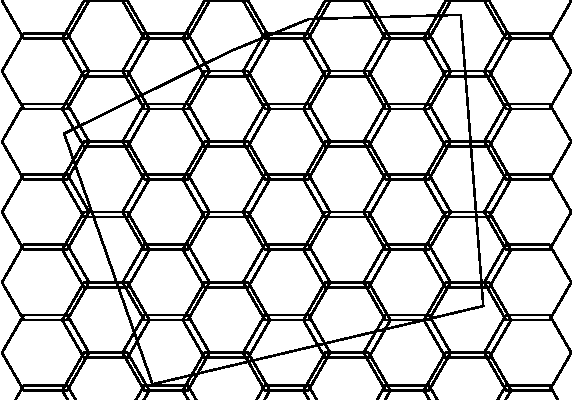
\includegraphics{README_files/figure-latex/unnamed-chunk-1-1.pdf}

\begin{Shaded}
\begin{Highlighting}[]
\NormalTok{cuad2 <-}\StringTok{ }\KeywordTok{st_as_sf}\NormalTok{(cuad)}
\NormalTok{cuad2 <-}\StringTok{ }\NormalTok{cuad2 }\OperatorTok
\StringTok{  }\KeywordTok{mutate}\NormalTok{(}
    \DataTypeTok{ENLACE=}\DecValTok{1}\OperatorTok{:}\KeywordTok{nrow}\NormalTok{(cuad2),}
    \DataTypeTok{AREASQM1=}\KeywordTok{st_area}\NormalTok{(geom) }\OperatorTok\StringTok{ }\NormalTok{units}\OperatorTok{::}\KeywordTok{drop_units}\NormalTok{())}
\NormalTok{cuad3 <-}\StringTok{ }\KeywordTok{st_intersection}\NormalTok{(cuad2, parque }\OperatorTok\StringTok{ }\NormalTok{st_union) }\OperatorTok
\StringTok{  }\KeywordTok{mutate}\NormalTok{(}\DataTypeTok{AREASQM2=}\KeywordTok{st_area}\NormalTok{(geom) }\OperatorTok\StringTok{ }\NormalTok{units}\OperatorTok{::}\KeywordTok{drop_units}\NormalTok{(),}
         \DataTypeTok{AREASQM_PCT=}\NormalTok{AREASQM2}\OperatorTok{/}\NormalTok{AREASQM1}\OperatorTok{*}\DecValTok{100}\NormalTok{)}
\end{Highlighting}
\end{Shaded}

\begin{verbatim}
## Warning: attribute variables are assumed to be spatially constant
## throughout all geometries
\end{verbatim}

\begin{Shaded}
\begin{Highlighting}[]
\NormalTok{pct_eleg <-}\StringTok{ }\DecValTok{40}
\NormalTok{cuad4 <-}\StringTok{ }\NormalTok{cuad2 }\OperatorTok
\StringTok{  }\KeywordTok{inner_join}\NormalTok{(}
\NormalTok{    cuad3 }\OperatorTok
\StringTok{      }\KeywordTok{filter}\NormalTok{(AREASQM_PCT }\OperatorTok{>=}\StringTok{ }\NormalTok{pct_eleg) }\OperatorTok
\StringTok{      }\KeywordTok{st_drop_geometry}\NormalTok{() }\OperatorTok
\StringTok{      }\KeywordTok{select}\NormalTok{(ENLACE, AREASQM2, AREASQM_PCT))}
\end{Highlighting}
\end{Shaded}

\begin{verbatim}
## Joining, by = "ENLACE"
\end{verbatim}

\begin{Shaded}
\begin{Highlighting}[]
\NormalTok{cuad4}\OperatorTok{$}\NormalTok{ENLACE <-}\StringTok{ }\DecValTok{1}\OperatorTok{:}\KeywordTok{nrow}\NormalTok{(cuad4)}
\NormalTok{cuad4}\OperatorTok{$}\NormalTok{ENLACE}
\end{Highlighting}
\end{Shaded}

\begin{verbatim}
##  [1]  1  2  3  4  5  6  7  8  9 10 11 12 13 14 15 16 17 18 19 20 21 22 23
## [24] 24 25 26 27 28
\end{verbatim}

\begin{Shaded}
\begin{Highlighting}[]
\NormalTok{cuad_final <-}\StringTok{ }\NormalTok{cuad4}
\KeywordTok{names}\NormalTok{(cuad_final)[}\KeywordTok{grepl}\NormalTok{(}\StringTok{'^geom$'}\NormalTok{, }\KeywordTok{names}\NormalTok{(cuad_final))] <-}\StringTok{ "geometry"}
\KeywordTok{st_geometry}\NormalTok{(cuad_final) <-}\StringTok{ "geometry"}
\NormalTok{cuad_final}
\end{Highlighting}
\end{Shaded}

\begin{verbatim}
## Simple feature collection with 28 features and 9 fields
## geometry type:  POLYGON
## dimension:      XY
## bbox:           xmin: 402697.2 ymin: 2041872 xmax: 403143.5 ymax: 2042260
## CRS:            32619
## First 10 features:
##    id     left     top    right  bottom ENLACE AREASQM1 AREASQM2
## 1   9 402697.2 2042190 402783.8 2042115      1 4871.393 2158.696
## 2  10 402697.2 2042120 402783.8 2042045      2 4871.393 4182.277
## 3  11 402697.2 2042050 402783.8 2041975      3 4871.393 2485.221
## 4  17 402757.2 2042157 402843.8 2042082      4 4871.393 4871.393
## 5  18 402757.2 2042087 402843.8 2042012      5 4871.393 4871.393
## 6  19 402757.2 2042017 402843.8 2041942      6 4871.393 4871.393
## 7  20 402757.2 2041947 402843.8 2041872      7 4871.393 3710.643
## 8  23 402817.1 2042190 402903.7 2042115      8 4871.393 4871.393
## 9  24 402817.1 2042120 402903.7 2042045      9 4871.393 4871.393
## 10 25 402817.1 2042050 402903.7 2041975     10 4871.393 4871.393
##    AREASQM_PCT                       geometry
## 1     44.31373 POLYGON ((402697.2 2042152,...
## 2     85.85383 POLYGON ((402697.2 2042082,...
## 3     51.01664 POLYGON ((402697.2 2042012,...
## 4    100.00000 POLYGON ((402757.2 2042120,...
## 5    100.00000 POLYGON ((402757.2 2042050,...
## 6    100.00000 POLYGON ((402757.2 2041980,...
## 7     76.17212 POLYGON ((402757.2 2041910,...
## 8    100.00000 POLYGON ((402817.1 2042152,...
## 9    100.00000 POLYGON ((402817.1 2042082,...
## 10   100.00000 POLYGON ((402817.1 2042012,...
\end{verbatim}

\begin{Shaded}
\begin{Highlighting}[]
\NormalTok{cuad_final <-}\StringTok{ }\NormalTok{cuad_final }\OperatorTok\StringTok{ }\KeywordTok{rename}\NormalTok{(}\DataTypeTok{a0_square_meters =}\NormalTok{ AREASQM1)}
\KeywordTok{plot}\NormalTok{(parque }\OperatorTok\StringTok{ }\NormalTok{st_geometry)}
\KeywordTok{plot}\NormalTok{(cuad_final }\OperatorTok\StringTok{ }\NormalTok{st_geometry, }\DataTypeTok{add=}\NormalTok{T)}
\end{Highlighting}
\end{Shaded}

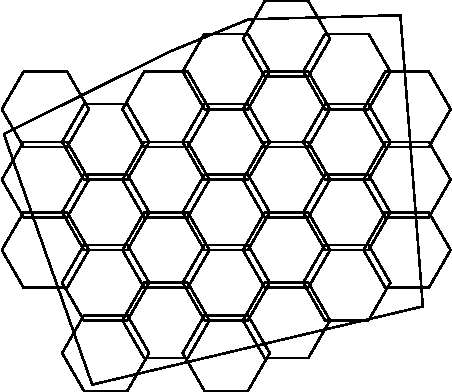
\includegraphics{README_files/figure-latex/unnamed-chunk-1-2.pdf}

\begin{Shaded}
\begin{Highlighting}[]
\CommentTok{# st_write(cuad_final, 'data/cuadricula-final.gpkg')}
\end{Highlighting}
\end{Shaded}

\hypertarget{referencias}{%
\section*{Referencias}\label{referencias}}
\addcontentsline{toc}{section}{Referencias}

\hypertarget{refs}{}
\leavevmode\hypertarget{ref-jose_ramon_martinez_batlle_2021_5694017}{}%
Batlle, J. R. M. (2021). geofis/forest-loss-fire-reproducible: First
release (Version v0.0.0.9000).
\url{https://doi.org/10.5281/zenodo.5694017}




\newpage
\singlespacing 
\end{document}